\documentclass{article}
\usepackage[utf8]{inputenc}
\usepackage{amsmath}
\usepackage{amssymb}
\usepackage{graphicx}

\begin{document}

\section*{Fast matrix multiplication with Eigen}
The lecture document presents the Strassen algorithm for two dense square matrices of size $n = 2^{k}$, $k \in \mathbb{N}$ with an asymptotic complexity better than $\mathcal{O}\left(n^{3}\right)$ (the normal complexity for multiplication of two $n \times n$ matrices). For the product of $\mathbf{A}, \mathbf{B} \in \mathbb{R}^{n,n}$ with $n = 2^{k}$ we define
\begin{equation*}
    \mathbf{A}\mathbf{B} = \mathbf{C} = \begin{bmatrix}
    \mathbf{C}_{11} & \mathbf{C}_{12} \\
    \mathbf{C}_{21} & \mathbf{C}_{22}
    \end{bmatrix}
\end{equation*}
We then compute the blocks of size $l \times l$ with $n = 2l$ for some $l \in \mathbb{N}$
\begin{align*}
    \mathbf{C}_{11} &= \mathbf{Q}_{0} + \mathbf{Q}_{3} - \mathbf{Q}_{4} + \mathbf{Q}_{6} \\
    \mathbf{C}_{21} &= \mathbf{Q}_{1} + \mathbf{Q}_{3} \\
    \mathbf{C}_{12} &= \mathbf{Q}_{2} + \mathbf{Q}_{4} \\
    \mathbf{C}_{22} &= \mathbf{Q}_{0} + \mathbf{Q}_{2} - \mathbf{Q}_{1} + \mathbf{Q}_{5}
\end{align*}
where $\mathbf{Q}_{k} \in \mathbb{R}^{l,l}$, $k = 0, \dots, 6$ are obtained from
\begin{align*}
    \mathbf{Q}_{0} &= \left(\mathbf{A}_{11} + \mathbf{A}_{22}\right) \cdot \left(\mathbf{B}_{11} + \mathbf{B}_{22}\right) \\
    \mathbf{Q}_{1} &= \left(\mathbf{A}_{21} + \mathbf{A}_{22}\right) \cdot \mathbf{B}_{11} \\
    \mathbf{Q}_{2} &= \mathbf{A}_{11} \cdot \left(\mathbf{B}_{12} - \mathbf{B}_{22}\right) \\
    \mathbf{Q}_{3} &= \mathbf{A}_{22} \cdot \left(-\mathbf{B}_{11} + \mathbf{B}_{21}\right) \\
    \mathbf{Q}_{4} &= \left(\mathbf{A}_{11} + \mathbf{A}_{12}\right) \cdot \mathbf{B}_{22} \\
    \mathbf{Q}_{5} &= \left(-\mathbf{A}_{11} + \mathbf{A}_{21}\right) \cdot \left(\mathbf{B}_{11} + \mathbf{B}_{12}\right) \\
    \mathbf{Q}_{6} &= \left(\mathbf{A}_{12} - \mathbf{A}_{22}\right) \cdot \left(\mathbf{B}_{21} + \mathbf{B}_{22}\right)
\end{align*}
We recursively apply this splitting process until we reach the base case for $n = 2$ and $l=1$ which gives us a recursion relation of (in each step we do $7$ smaller matrix multiplications and a computational effort of $\mathcal{O}\left(n^{2}\right)$ for the matrix additions.)
\begin{equation*}
    \mathrm{T}\left(n \right) \leq 7\cdot\mathrm{T}\left(\frac{n}{2}\right) + \mathcal{O}\left(n^{2}\right)
\end{equation*}
Let us look at the Master theorem.
 \begin{figure}[!hbt]
    \centering
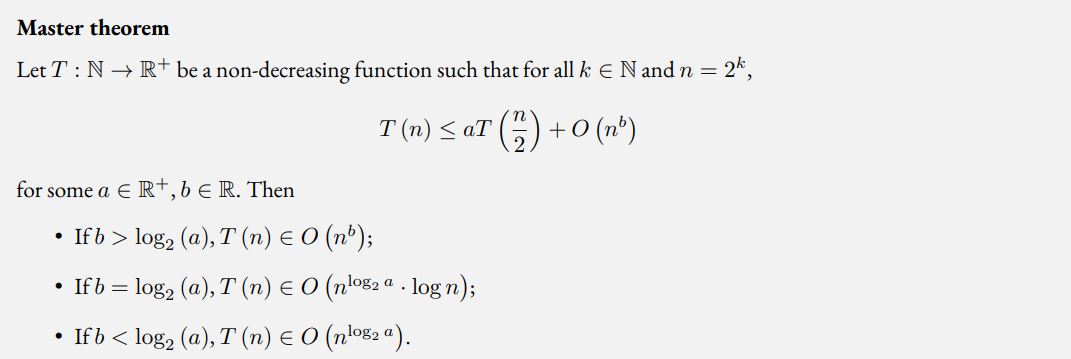
\includegraphics[width=1.0\linewidth]{MasterTheorem.png}
\end{figure}

\noindent This gives us $a = 7$ and $b = 2$ and thus $\log_{2}\left(7\right) = 2.805\dots > 2 = b$.

\pagebreak 


\noindent The resulting asymptotic complexity is thus  
\begin{equation*}
    \mathrm{T}\left(n\right) \in \mathcal{O}\left(n^{\log_{2}\left(7\right)}\right)
\end{equation*}
\subsection*{1-4.a}
We are now tasked with implementing a recursive function \verb|strassenMatMult| that uses Strassen algorithm to mulitply two \textbf{square} matrices $\mathbf{A}, \mathbf{B} \in \mathbb{R}^{n,n}$ with $n = 2^{k}$ for some $k \in \mathbb{N}$. We implement the exact algorithm presented above and get first the following wrapper function that checks if the input is valid and a helper function that does the actual work.

 \begin{figure}[!hbt]
    \centering
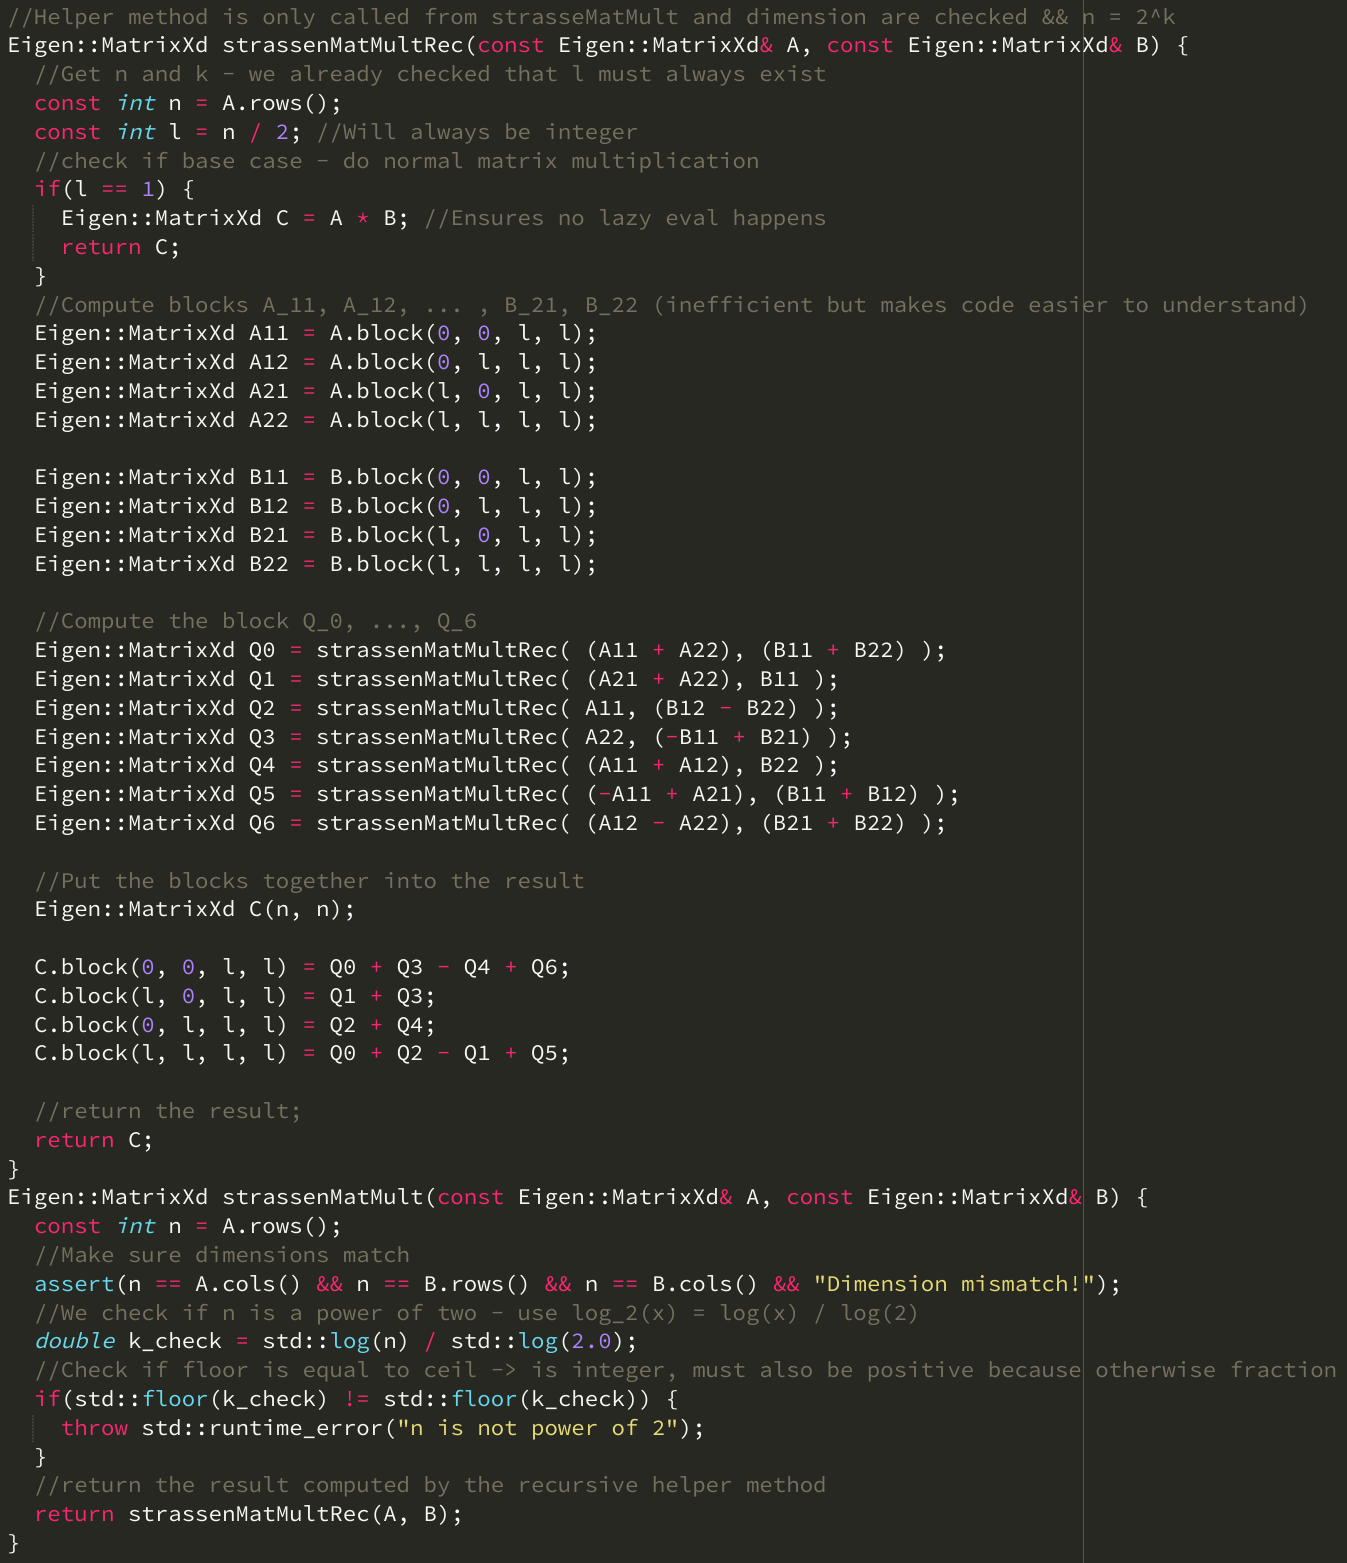
\includegraphics[width=1.0\linewidth]{StrassenMatMult.png}
\end{figure}

\subsection*{1-4.b}
We are now tasked with writing a method that checks if the code written in 1-4.a computes the correct result by comparing it to the built-in matrix multiplication. Given two results $\mathbf{C}_{1}$ and $\mathbf{C}_{2}$ we cannot just compare the entries are the results will suffer from round-off error. What we can do is to use the built-in Frobenius norm in Eigen given by
\begin{figure}[!hbt]
    \centering
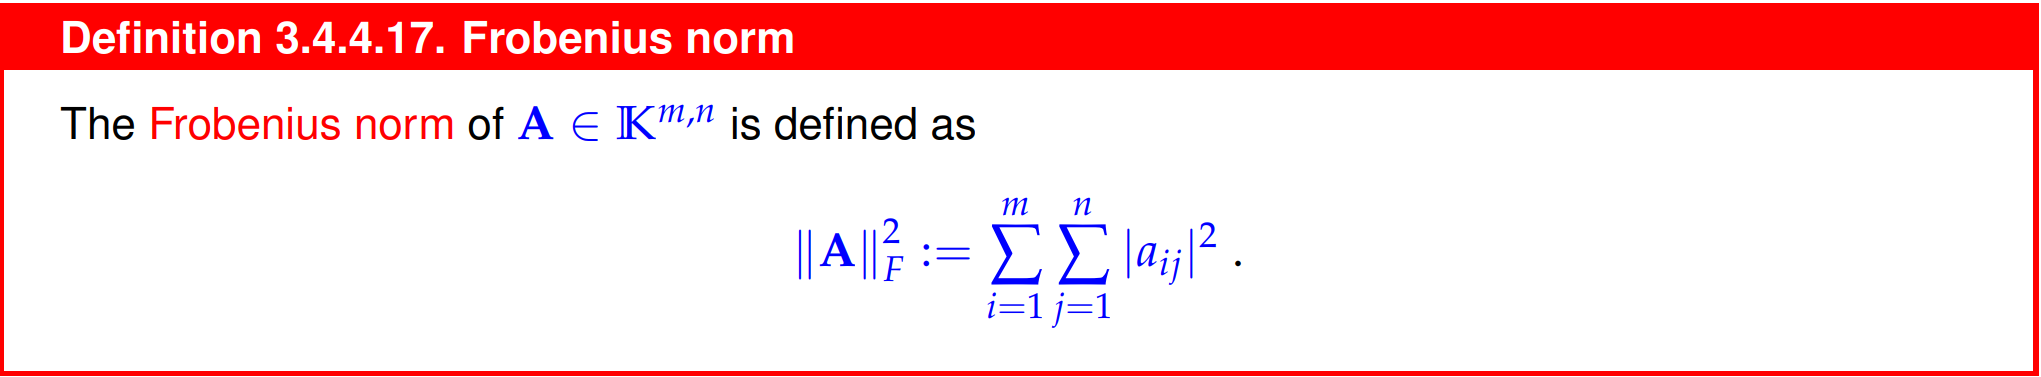
\includegraphics[width=1.0\linewidth]{FrobeniusNorm.png}
\end{figure}

\noindent and compare the two matrices in that way while (as always) taking the result we consider to be correct as a reference combined with some tolerance factor $\tau$. Here $\mathbf{C}_{1}$ is the result computed from the built-in Eigen matrix multiplication.
\begin{equation*}
    \left\lVert \mathbf{C}_{1} - \mathbf{C}_{2}\right\rVert_{\mathrm{F}} < \tau \cdot \left\lVert \mathbf{C}_{1} \right\rVert_{\mathrm{F}} 
\end{equation*}

\noindent This produces the following code
 \begin{figure}[!hbt]
    \centering
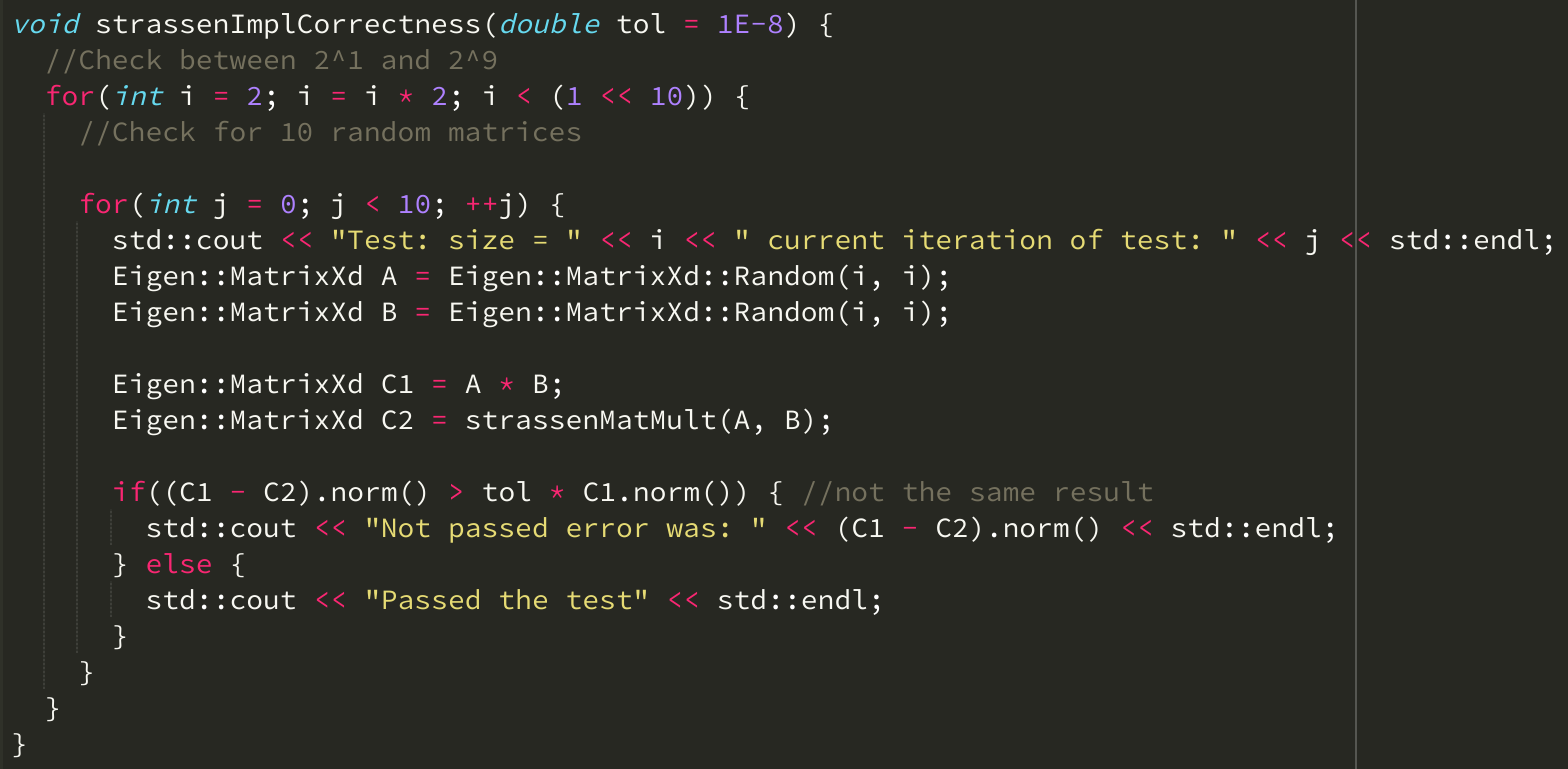
\includegraphics[width=0.9\linewidth]{1-4.b.png}
\end{figure}
\subsection*{1-4.c}
As this exercises brings little value to understanding the concepts, only a few notes, here we again use the \verb|Timer| utility which we can start with \verb|start()| and stop with \verb|stop()|, however taking duration does not work here as it would return the total time the timer did run, here it would hence sum up (view solution given) all repetitions (given by \verb|repetitions|) and not the average. We return \verb|min()| which will give us the minimum time that elapsed between a \verb|start| and \verb|stop| call for the specific timer. We do create the timers for each test size hence \verb|min| always return ths value only for the current test size.

